To test the \cshia~ architecture  we utilized industry standard IPs provided with no cost for academic purposes, the target processor to receive the security updates was the Leon3, any processor with an AMBA2 interface  could be used since the goal of this work is to test how easy the implementation fits an already existing design and  the impact on the performance. This chapter shows the prototype hardware setup in Section \ref{sec:hardware_setup} giving details of the design kit used for this implementation and \leon, the processor selected to host \cshia,  and in Section \ref{sec:gaisler_tools} the tools used to make this implementation work and its features are presented. 

\mario{Apresentar a organização do capítulo. Sempre. No início do capítulo. Ajuda o leitor a se localizar.} \augusto{colocado junto ao texto}

\section{Hardware setup}
\label{sec:hardware_setup}
 \begin{figure}[!ht]
    \centering
    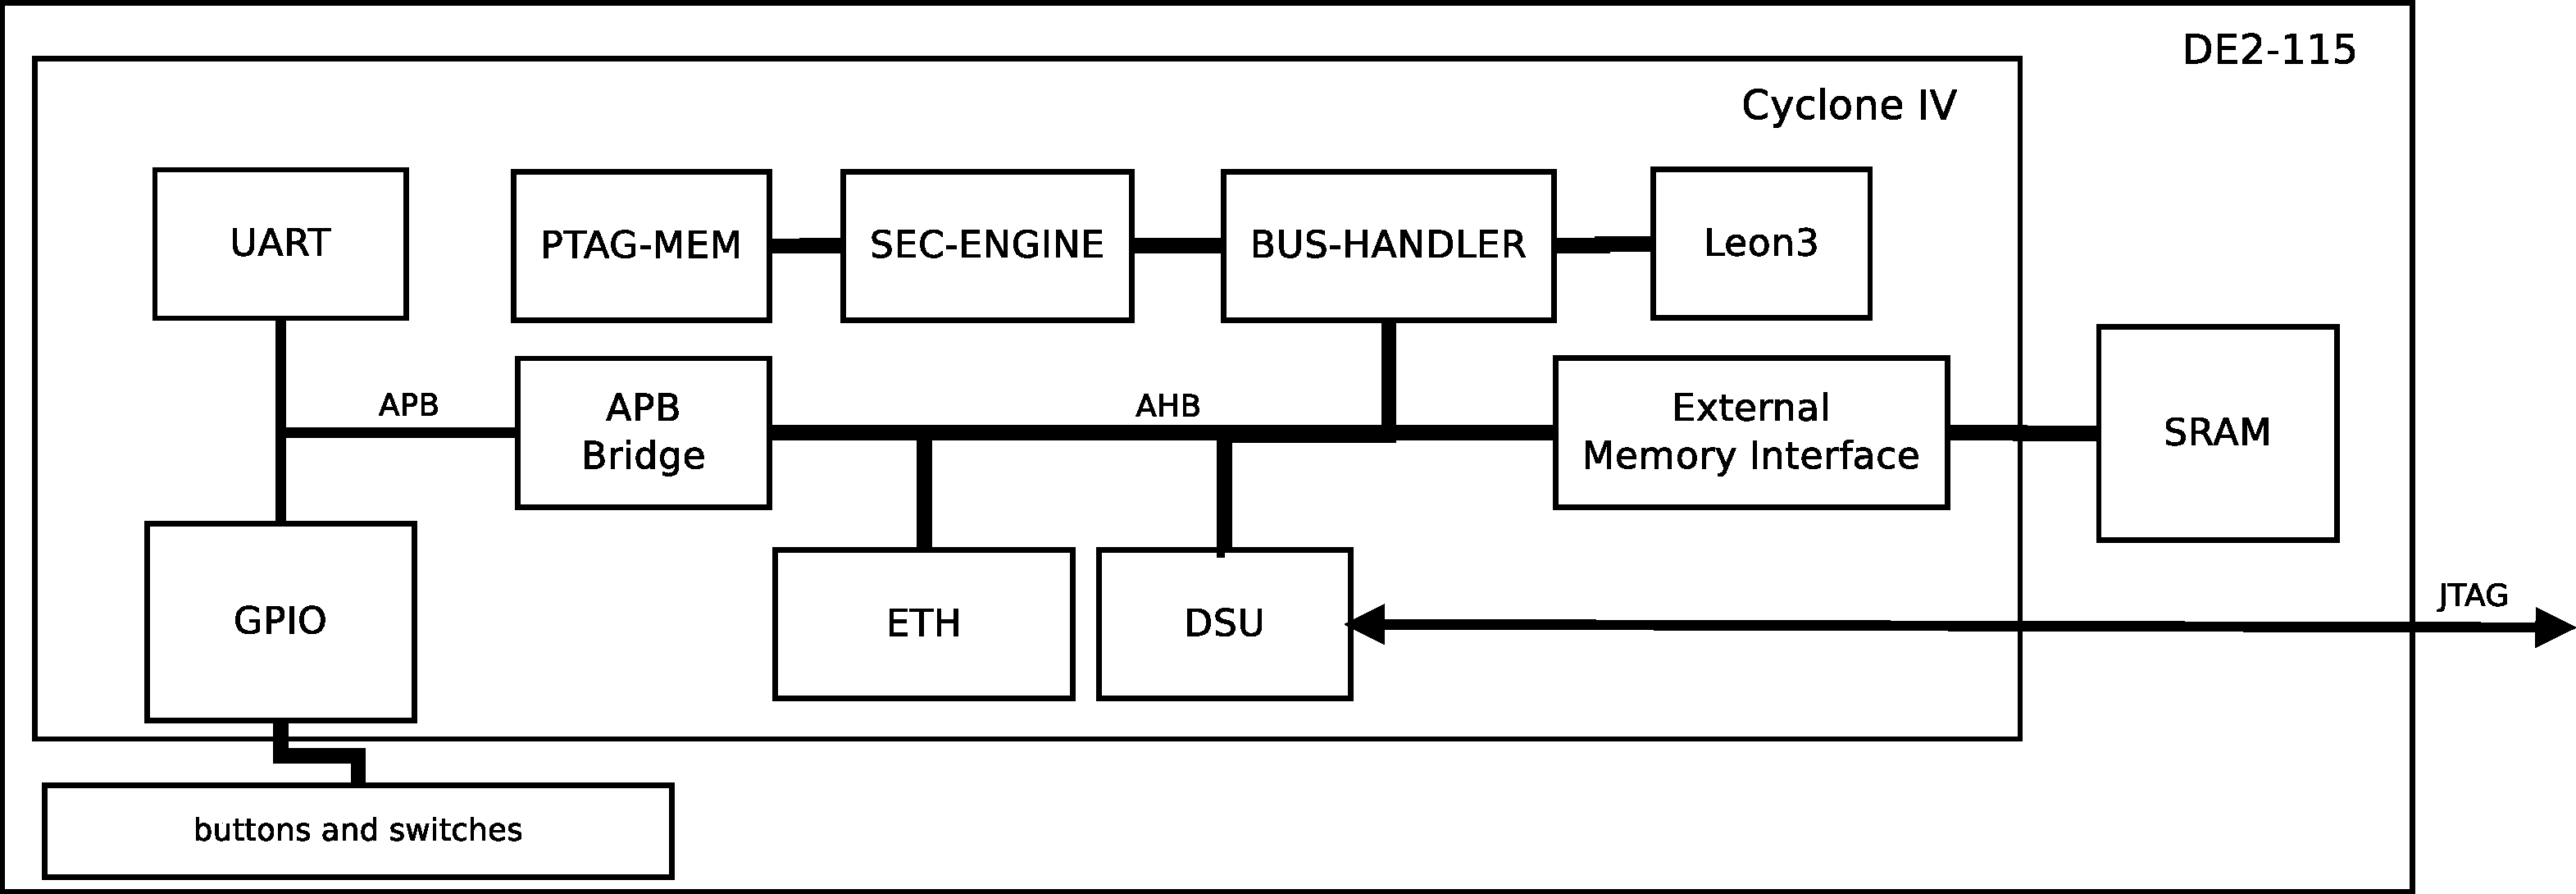
\includegraphics[width=1\textwidth]{figures/pdf/leon_amba_new.pdf}
    \caption{\cshia integrated with the DE2-115 kit ,with \leon~, DSU and all presented security components. }
    \label{fig:leoninamba}
\end{figure}

We chose the \leon~platform from Cobham Gaisler~\cite{Leon} to implement \cshia. \leon~is a \vhdl~implementation of a SPARC V8 processor with configurable parameters, which together with some additional IP cores provide a suitable solution for embedded systems. In addition, \leon~has a free version for academic purposes that include sophisticated debugging tools, and it is available for a variety of \fpga~Development kits. Gaisler keeps an email list for support and constant updates are provided. All these features are interesting because \cshia~can be an extension of the platform available to the research community, and which also has solid design choices since \leon~is a product available to the industry.


The implementation is based on Figure \ref{fig:cshiaexpanded} and better visualized in Figure \ref{fig:leoninamba}. \leon's processor (the core) is connected through the main memory by a \amba~Bus version 2.0. In our modification, the processor's \io~master bus connects it to \handler, which then provides a new \io~master bus for the rest of the components in the platform. Thus, \handler~is transparent to all components of the platform, even the core. One of the components that is specific of \leon's platform is the Debug Support Unit (\dsu), which allows a designer using a debug host (such as a computer) to connect to development kits running \leon. Through the debugging connection, a program can be loaded to the \fpga~memory, started, paused, among other useful functions.



\begin{table}[!h]
  \center
  \caption{\cshia~\fpga~implementation configuration.} 
  \label{tab:config}
  \footnotesize
  \begin{tabular}{|l|l|}
%\    \noalign{\hrule height 1pt}
%\    \rowcolor{lightgray}
    \hline
      Component & Parameter\\ 
    %\noalign{\hrule height 0.75pt}
    \hline
    \hline
      \leon~Processor & \\
      \hspace{0.25in} Frequency & 50 MHz\\
      \hspace{0.25in} Instruction Cache & 16 KB\\
      \hspace{0.25in} Data Cache & 16 KB\\
      \hspace{0.25in} Cache Line Size & 256 bits\\
      \hspace{0.25in} Memory Word & 32 bits\\
    \hline
      Code and Data Memory & Up to 128 MB\\
      \hspace{0.25in} Code Start Address & \texttt{0x40000000}\\
      \hspace{0.25in} Data Start Address 1 & \texttt{0x40013000}\\
      \hspace{0.25in} Data Start Address 2 & \texttt{0x40023000}\\
    \hline
      \handler~Buffer & 128 Bytes\\
    \hline
      \fuzzy & \\
      \hspace{0.25in} \ecc & (127,64,10)-\bch\\
      \hspace{0.25in} \pufs & 64 $\times$ 64-bit Arbiter \pufs\\
    \hline
      \ptaggen & \\
      \hspace{0.25in} \prf & \siphash-2-4\\
      \hspace{0.25in} \siphash-2-4 key & 128 bits\\
      \hspace{0.25in} \ptag~generation & 10 cycles\\
      \hspace{0.25in} \ptag~length & 64 bits\\
    \hline
      \ptag~Memory & 216,064 bytes\\
      \hspace{0.25in} Code and Data \ptags & 18816 words of 64 bits\\ 
      \hspace{0.25in} \mt~\ptags & 8192 words of 64 bits\\ 
      \hspace{0.25in} Data coverage & 512 KB\\
      \hspace{0.25in} Total coverage & 588 KB\\
    \hline
      \pmmu & \\
      \hspace{0.25in} Time Stamp Memory & $2^{14}$ timestamps\\
      \hspace{0.25in} Time Stamp Length & 16 bits\\
      \hspace{0.25in} \ptag~Cache & 4 KB \\
      \hspace{0.25in} \pmmu~Buffer for \mt & 2 * number of cache lines\\
    \hline
  \end{tabular}
%\vspace*{-12pt}
\end{table}
We implemented \cshia~in an Altera \fpga~Development Kit DE2-115. The parameters of the processor and \cshia~are in Table \ref{tab:config}. The Altera's kit allows the processor to run at 50 MHz. The total amount of SDRAM memory dedicated to \leon~is 128 MB. As convention all programs starts by its \texttt{.text} segment (code) at the address \texttt{0x40000000}. We set \texttt{.data} segment (data) to start at \texttt{0x40013000}, or at \texttt{0x40023000}, depending on the size of the code segment. As described in the previous section, \handler~has a buffer that stores memory words. When these words form a memory block, it is handed to \seceng. We set the size of this buffer to 4 cache lines, which gives a total of 128 bytes. The 128-bit \siphash's key is extracted from 64 Arbiter \pufs~(\apufs). Although any \puf~could be used, due to the simplicity of design we chose the \apuf~as a proof of concept. Each \apuf~has a 64-bit challenge input. \ptag~generation lasts 10 cycles, between \seceng~request and \ptaggen~reply.


Continuing to look at Table \ref{tab:config}, the \ptagmem~uses internal memory of the \fpga. This option arose due to limiting options available in the kit. Because we wanted to design a 64-bit bus memory, no better option than internal memory was available. The \sram~of the kit only allowed 16-bit words. We also could not increase the frequency of the \sram~using PLLs since its maximum frequency was limited to 125 MHz, and, to simulate a 64-bit bandwidth, we would need at least a \sram~operating at 200 MHz. The option for \fpga~internal memory limited our coverage to a maximum of 512 KB of data memory, which resulted in a memory overhead of 36 \% (code, data, and \mt). In addition, to reduce unused memory words in \ptagmem, we split it into two. This allowed to create an easy decoder to separate \ptags~of memory blocks from those of chunks of \ptags. 

%Due to the high utilization of internal memory, timestamp memory became limited to $2^{14}$ 16-bit words to cover the 512 KB of data memory. This represents 5.4\% of the total 588 KB main memory coverage. The \ptagmem~utilization for this solution was up to 147 KB (code and data), or 25\% overhead. Table \ref{tab:config} also shows the \ptag~cache's configuration. Since this cache is an internal memory as well, it was limited to 4 KB. That limitation did not prevent us of evaluating the cache in multiple configurations. We evaluated this cache in different configurations of lines, set associativity, and replacement policies. Finally, as previously discussed, \pmmu~requires a buffer to stall a \ptag~cache write or read while an eviction is required. We calculated that this buffer needs to be at most 2 times the number of lines in \ptagcache. 

%One last information about our \fpga~\cshia~implementation is that it had three modes of operation. In the first mode, called \baseline, the \handler~is disabled and all security-specific hardware is bypassed. A second mode, the \timestamp, activates \pmmu~for timestamps only. Finally, the third mode, \textit{\cshia-MT}, disables timestamps and activates the cache in \pmmu~for supporting the Merkle Tree implementation. Being able to switch between those modes only using switch keys of the development key helped us in debugging and evaluating the performance of the architecture.


\section{GAISLER Tools}
\label{sec:gaisler_tools}
Together with \leon~Gaisler also provides simulation and debug tools,  the simulators to test software while the hardware is being developed and the debug software named  GRMON to load and debug programs directly on hardware. Whit GRMON one can access all masters and slaves on the bus and perform debug operations like inserting breakpoints for instance.  This section gives us an overview of the GRMON features and an explanation about how the debug works.

\subsection{Overview}
 GRMON \cite{GRMON} is a general debug monitor and control software that can be used after one SoC design, using GRLIB IP Library cores is loaded to an \fpga~or after being manufactured as an ASIC.  With the GRMON console, it is possible to download and execute \leon~applications, and it  also includes the following features:
\begin{itemize}
 \item Read/write access to all system registers and memory
 \item Built-in disassembler and trace buffer management
 \item Downloading and execution of LEON applications
 \item Breakpoint and watchpoint management
 \item Remote connection to GNU debugger (GDB)
 \item Support for USB, JTAG, RS232, PCI, Ethernet and SpaceWire debug links
\end{itemize}

\subsection{Debug}

The GRMON debug monitor is intended to debug SOCs designs based on the LEON processor. The monitor connects to a dedicated debug interface on the target hardware, through which it can perform read and write cycles on the on-chip bus (AHB).LEON3 also supports JTAG, ethernet and spacewire (using the GRESB ethernet to spacewire bridge) debug interfaces. On the target system, all debug interfaces are realized as AHB masters with the debug protocol implemented in hardware. There is thus no software support necessary to debug a LEON system, and a target system does in fact not even need to have a processor present.

 \begin{figure}[ht]
    \centering
    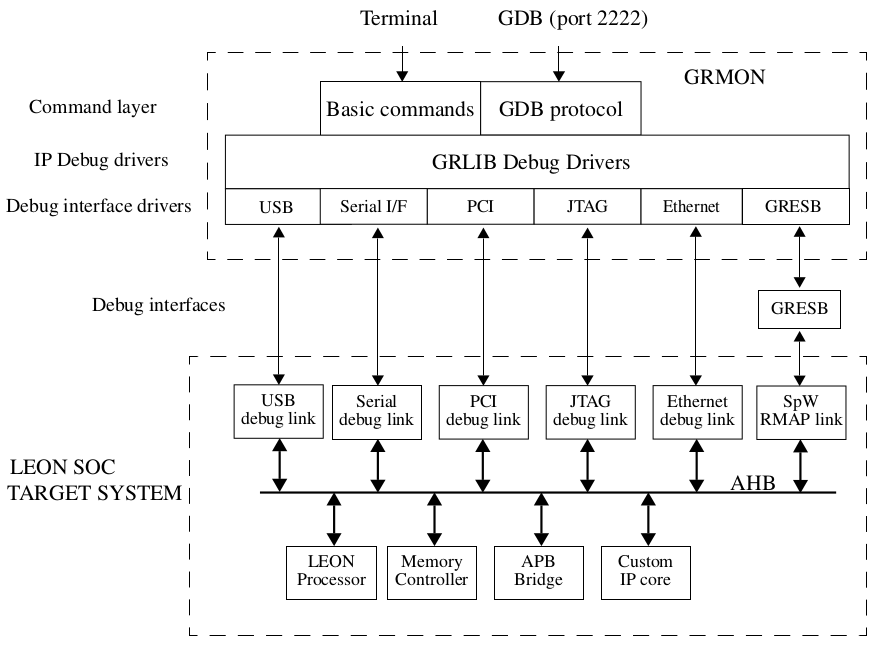
\includegraphics[width=0.75\textwidth]{figures/others/grmon_ex.png}
    \caption{GRMON  Interface }
    \label{fig:grmon_int}
\end{figure}
GRMON can operate in two modes: command-line mode and GDB mode. In command-line mode, GRMON
commands are entered manually through a terminal window. In GDB mode, GRMON acts as a GDB gateway
and translates the GDB extended-remote protocol to debug commands on the target system. As illustrated in Figure \ref{fig:grmon_int} GRMON is implemented using three functional layers: command layer, debug driver layer, and debug interface layer. The command layer consist of a general command parser which implements commands that are independent
of the used debug interface or target system. These commands include program downloading and flash programming.
The debug driver layer implements custom commands which are related to the configuration of the target system. 
GRMON scans the target system at startup, and detects which IP cores are present and how they are configured. For each supported IP core, a debug driver is enabled which implements additional debug commands for the specific core. Such commands can consist of memory detection routines for memory controllers, or program debug commands for the LEON processors. The debug interface layer implements the debug link protocol for each supported debug interface. The protocol depends on which interface is used, but provides a uniform read/write interface to the upper layers. Which
interface to use for a debug session is specified through command-line options during the start of GRMON.



